%%%%
\section{Fluorescência de Raios X}

Para determinação e quantificação das concentrações elemenares (número atômico $Z>10$)
foi utilizada a técnica não-destrutiva de \textit{Fluorescência de Raios X}.

\textit{Fluorescência de Raios X} é um método analítico quali-quantitativo, 
multielementar, que mede os raios-X característicos emitidos dos átomos da amostra, 
depois de também serem irradiados por Raios X. Não exige pré-tratamento químico
das amostras.

Existem 3 Tipos de fluorescências de raios X: dispersão em energia,
dispersão por comprimento de onda e reflexão total.
O usado nessa pesquisa foi o 
\textit{Fluorescência de Raios X por dispersão em energia}.

A figura \ref{fig:shimadzu_atomo} ilustra classicamente o que ocorre com
o átomo ao ser excitado.

\begin{figure}[H]
\begin{center} 
  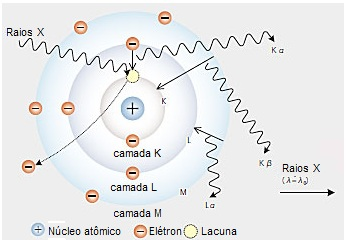
\includegraphics[width=0.5\textwidth]{../inputs/images/shimadzu_atomo.jpg}
  \caption{Shimadzu - Figura que acompanha o manual do XRF-ED \label{fig:shimadzu_atomo}}
   % http://www.shimadzu.com.br/analitica/produtos/elemental/raios_x/eds/images/edx-7000_8000-2.jpg
\end{center}
\end{figure}

O feixe de raios x incidente, neste caso produzido por tudo de raios X, 
expulsa os elétrons das camadas mais internas $K$ e $L$, produzindo vacâncias. 
Um átomo com vacância é instável e rapidamente elétrons das camadas 
mais externa preenchem as vacâncias estabilizando o átomo.

As transições dos elétrons das camadas mais externas para as camadas
$K$ e $L$ liberam Raios X característicos do átomo em questão. 

Transições da camada $L$ para $K$ são do tipo $K\alpha$, de $M$ para $K$ 
são $K\beta$ e de $M$ para $L$ são $L\alpha$ ou $L\beta$. 
A camada $L$ possue 3 e a camada $M$ 5 subníveis o que
resulta em inúmeras possibilidades de transições, sendo que algumas transições
proibidas. 

A \textit{notação de Siegbahn} permite identificarmos melhor os subníveis
de origen e destino, por exemplo, transição de $M_{IV}$ para $L_{III}$ é uma transição do 
tipo $L\beta_1$ \cite{jenkins1991}, outras possíveis pode ser vista na
figura \ref{fig:siegbahn}. 

\begin{figure}[H]
\begin{center} 
  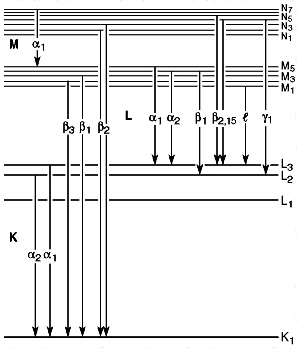
\includegraphics[width=0.5\textwidth]{../inputs/images/Siegbahn.jpg}
  \caption{Transições - artigo \cite{jenkins1991}  \label{fig:siegbahn}}
\end{center}
\end{figure}

Entretanto, há transições com energias são tão próximas 
que são indistinguiveis para os detectores (semicondutores) 
utilizados, sendo assim, neste trabalho vamos chamar apenas de 
transições tipo $K$ e $L$.

%%%%
\subsection{Fluorescência de Raios X por dispersão em energia}

A \textit{Fluorescência de Raios X por dispersão em energia} (\textbf{XRFED}).
usa detectores de semicondutores capaz de discriminar energia 
próximas, onde a distinção dos fótons é feita pela amplitude do pulso 
eletrônico produzido no detector, pois os pulsos eletrônicos são
proporcionais às energias dos raios X. 

O detector mais empregado é o de silício ativado com lítio $Si(Li)$.



E a figura \ref{fig:xrfed_iag} ...

\begin{figure}[H]
\begin{center}
  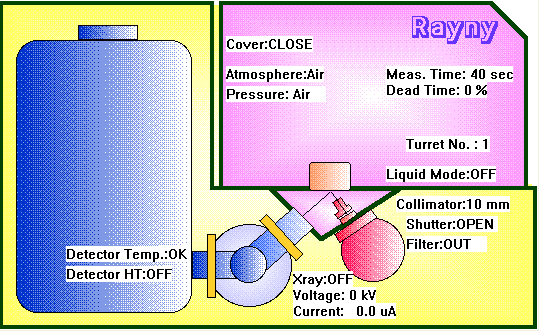
\includegraphics[scale=0.4]{../inputs/images/edx_iag_monitor.png}
  \caption{Fluorescência de Raios X por dispersão em energia do IAG USP - \label{fig:xrfed_iag}}
\end{center}
\end{figure}

%%%%
\subsection{Calibração}

O método \textit{PIXE (Particle Induced X-Ray Emission)}, 
também comumente usado em análises ambientais, usa feixe de íons 
(prótons ou alfas) para excitação dos átomos das amostras.

\begin{figure}[H]
\begin{center} 
  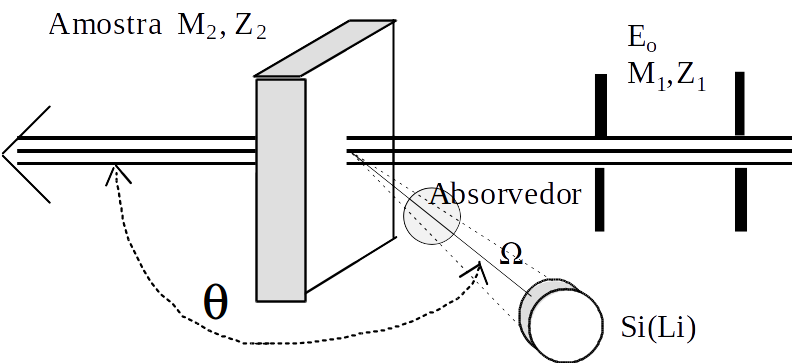
\includegraphics[width=0.8\textwidth]{../inputs/images/arranjopixe.png}
  \caption{Arranjo experimental básico para análise de método PIXE 
           \cite{tabacniks2000} \label{fig:arranjopixe}}
\end{center}
\end{figure}

Baseado no arranjo experimental da figura \ref{fig:arranjopixe} e
considerando o filtro fino (alguns $\mu m$),
\cite{tabacniks2000} chega na equação \ref{eq:npixe} para quantidade de Raios X
contadas no detector. 

\begin{equation}
  \label{eq:npixe}
  N(Z) = \frac{\Omega}{4\pi} \sigma \zeta T t_z \frac{Q}{qe}
\end{equation}

Sendo que, o número de raios X detectados $N(Z)$ é proporcional à 
densidade (massa ou átomos por área) $t_Z$ e a carga coletada $Q$.
$Z$ é espécie química, $\zeta$ é a eficiência do detector, 
$\sigma_x$ é a secção de choque, $\Omega$ é o ângulo sólido, 
$T$ é a transmitância para raios-X em caso de uso de absorvedores 
(colocados entre a amostra e o detector), $q$ é o estado de carga da 
partícula incidente e $e$ é a carga do elétron \cite{tabacniks2000}.

Para resolver a equação \ref{eq:npixe}, parâmetros do arranjo experimental
deveriam ser conhecidos: $\Omega$, $\sigma$, $\zeta$ e $T$. 

Porém, se usarmos filtros de calibração (comprados ou produzidos) 
com $t_z$ conhecidos, podemos agrupar todas variáveis
do arranjo experimental em uma única, chamada de fator de resposta $R(Z)$.

Assim, a equação \ref{eq:npixe} se torna \ref{eq:contagem}

\begin{equation}
  \label{eq:contagem}
  N(Z) = R(Z) I\Delta_t \frac{m}{a}
\end{equation}

$R(Z)$ é o fator de resposta, $I\Delta_t$ é a carga efetiva expressa
em termos da corrente e do tempo de análise e $\frac{m}{a}$ é a 
densidade $t_z$






%86 # Y and X were measured
%187 # 
%188 # $[X]A=[Y]$
%189 # 
%190 # We will adjust a A for equation above and call it Ã, but before we have to calculate the covariance of the coeficients $V_Ã$:
%191 # 
%192 # $V_Ã = (X^T V_Y^{-1} X)^{-1}$
%193 # 
%194 # and
%195 # 
%1%96 # $Ã = V_Ã X^T V_Y^{-1} Y$
%197 # 
%198 # Now, we can calculate the new values of Y from $V_Ã$ to all atomic numbers in covered region $X_{adjusted}$:
%199 # 
%200 # $[X_{adjusted}]Ã=[Y_{adjusted}]$
%201 # 
%202 # The error desired is the square roots of diagonal of matrix covariance of Ycalculed $C_{Yadjusted}$.
%203 # 
%204 # $C_{Y_{adjusted}} = X_{adjusted} V_Ã X_{adjusted}^T$

\begin{equation}
\begin{split}
F = \{F_{x} \in  F_{c} &: (|S| > |C|) \\
 &\quad \cap (\text{minPixels}  < |S| < \text{maxPixels}) \\
 &\quad \cap (|S_{\text{conected}}| > |S| - \epsilon) \}
\end{split}
\end{equation}

%%%%
\subsection{Limite de Detecção}

Densidade mínima para haver detecção da espécie. % como determina para XRF?

Amostra espessas apresentam o efeito matriz, ou seja, interações dos 
raios X característicos com os elementos da amostras, causando 
absorção do raios X ou mesmo reforço de raios X.





